\chapter{Listings}

\lstset{language=Java}
\lstinputlisting[captionpos=b,label={app:feedbacks},caption={Die Liste von Benutzerfeedbacks}]{Listings/feedbacks.json}

\clearpage
\chapter{Tabellen}

\begin{table}
\begin{tabular}{|c|c|c|c|c|}
\hline 
• & helpQuality & qualityRating\_newspapers & qualityRating\_misc & speedRating \\ 
\hline 
mitie-nerchain-pig & 3.23 & 1.98 & 1.45 & 4.09 \\ 
\hline 
mitie-nerchain-tiger & 3.15 & 1.25 & 2.09 & 3.8 \\ 
\hline 
pig-nerchain & 3.05 & 1.31 & 2 & 3.87 \\ 
\hline 
stanford-nerchain-both & 3.07 & 1.23 & 1.95 & 4.05 \\ 
\hline 
stanford-nerchain-dewac & 3.25 & 2.11 & 1.41 & 4.16 \\ 
\hline 
stanford-nerchain-hgc & 3.11 & 1.34 & 1.86 & 4.16 \\ 
\hline 
tiger-nerchain & 3.34 & 1.93 & 1.39 & 3.98 \\ 
\hline 
\end{tabular} 
\caption{Evaluierung}
\label{app:RESULTS}
\end{table}

\clearpage
\chapter{Screenshots}

\begin{figure}
\centering
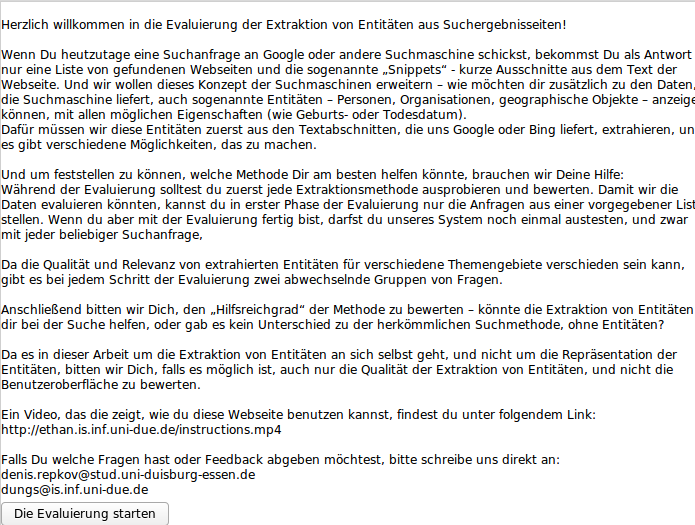
\includegraphics[width=1.0\textwidth]{Bilder/evalstep01.png}
\caption{''Einleitung in die Evaluierung''}
\label{app:evalstep01}
\end{figure}

